\documentclass{beamer}

\usepackage{amsmath}
\usepackage{amssymb}
\usepackage{tikz}
\usepackage{tikz-cd}

% To display speaker notes on a second screen, uncomment the two lines below:
% \usepackage{pgfpages}
% \setbeameroption{show notes on second screen=right}

\usetheme{default}
\setbeamertemplate{navigation symbols}{}

\title{Constructing Quotient Inductive Types}
\subtitle{Why quotients can be harder than they look}
\author{Christina O'Donnell\\[4pt]
  \footnotesize Joint work with Thorsten Altenkirch}
\date{EPSRC DTP \& DLA Research Showcase 2026}

\begin{document}

% ---------------------------------------------------------------------------
% Slide 0: Title
% ---------------------------------------------------------------------------
\begin{frame}
  \titlepage
\end{frame}

% ---------------------------------------------------------------------------
% Slide 1: Question
% ---------------------------------------------------------------------------
\begin{frame}{Question}
  \begin{center}
    \Large
    Can we construct symmetric infinitely-branching trees,
    without making infinitely many choices?
  \end{center}

  \vspace{1em}
  \begin{center}
  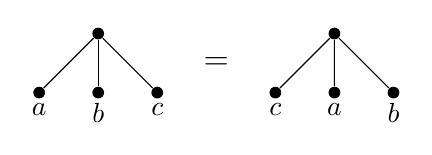
\begin{tikzpicture}[scale=0.75, every node/.style={inner sep=1.5pt}]
    \node (r1) at (0,0) [circle,fill,minimum size=4pt] {};
    \node (a1) at (-1,-1) [circle,fill,minimum size=4pt,label=below:$a$] {};
    \node (b1) at (0,-1) [circle,fill,minimum size=4pt,label=below:$b$] {};
    \node (c1) at (1,-1) [circle,fill,minimum size=4pt,label=below:$c$] {};
    \draw (r1) -- (a1);
    \draw (r1) -- (b1);
    \draw (r1) -- (c1);

    \node at (2, -0.5) {\large $=$};

    \node (r2) at (4,0) [circle,fill,minimum size=4pt] {};
    \node (c2) at (3,-1) [circle,fill,minimum size=4pt,label=below:$c$] {};
    \node (a2) at (4,-1) [circle,fill,minimum size=4pt,label=below:$a$] {};
    \node (b2) at (5,-1) [circle,fill,minimum size=4pt,label=below:$b$] {};
    \draw (r2) -- (c2);
    \draw (r2) -- (a2);
    \draw (r2) -- (b2);
  \end{tikzpicture}
  \end{center}


  \begin{center}
    \normalsize
    Equivalently: can we construct permutation-invariant trees in type
    theory?
  \end{center}

  \note{%
    Timing: 0:45.

    This talk is about a problem in the foundations of formal mathematics.

    The example I want to start with is a tree where the order of the
    children does not matter.

    So a node with children \(a,b,c\) should be the same as a node with
    children \(c,a,b\).

    Mathematically, this sounds innocent: we just identify trees that
    differ by a permutation of their children.

    But constructively, there is a catch.

    If we first quotient the trees, then each child is no longer given by
    a concrete tree. It is given only by an equivalence class of trees.

    To build a new raw node, we would need to pick a representative tree
    from each equivalence class.

    For finitely many children, this representative-picking step can often
    be hidden.

    But for a node with infinite children, we would need to make
    infinite choices at once.

    That is exactly the shape of a choice problem.

    So the question for this talk is: can we build these permutation
    invariant trees, and types like them, constructively inside type theory?
  }
\end{frame}

% ---------------------------------------------------------------------------
% Slide 2: Outline
% ---------------------------------------------------------------------------
\begin{frame}{Talk outline}
  Aim of my research:

  \begin{center}
    \large
    Can we construct quotient inductive types (QITs) inside type theory?
  \end{center}

  \begin{itemize}
    \item Type theory and constructive formalisation
    \item Quotients and quotient inductive types by example
    \item Why the obvious construction fails
    \item Where weak choice enters
    \item My contribution: a positive result for depth-preserving examples
    \item What remains open
  \end{itemize}

  \note{%
    Timing: 1:00.

    Here is the plan.

    I will first explain what type theory is and why constructivity matters
    for formalisation.

    Then I will introduce quotients and quotient inductive types by example.

    After that I will show why the obvious construction fails.

    I will then explain where a weak form of choice enters the existing
    general construction.

    Finally I will state my contribution: for a simple class of examples,
    including symmetric trees, we can recover the construction relative to an
    extensional ordinal basis.
  }
\end{frame}

% ---------------------------------------------------------------------------
% Slide 3: What is type theory?
% ---------------------------------------------------------------------------
\begin{frame}{What is type theory?}
  Type theory is a foundation for mathematics and computation.

  \medskip

  It is used in proof assistants such as:
  \[
    \text{Lean}
    \qquad
    \text{Agda}
    \qquad
    \text{Rocq}
  \]

  \medskip

  In a proof assistant, mathematical objects are represented by types,
  and proofs are checked by a computer.

  \medskip

  \begin{center}
    \large
    My work asks: which types can we build without adding extra axioms?
  \end{center}

  \note{%
    Timing: 1:30.

    Type theory is one of the foundations used for computer-checked
    mathematics.

    Systems such as Lean, Agda, and Rocq use type-theoretic ideas to let
    us define mathematical objects and check proofs about them.

    In this setting, a mathematical construction is not just something we
    describe informally.

    We want it to be something that can be built inside the system.

    So the question I care about is: when we introduce a new kind of type,
    are we really constructing it, or are we secretly adding a new axiom?
  }
\end{frame}

% ---------------------------------------------------------------------------
% Slide 4: Why constructivity matters
% ---------------------------------------------------------------------------
\begin{frame}{Why constructivity matters}
  Constructive mathematics distinguishes:

  \[
    \text{``there exists an object''}
    \qquad\text{from}\qquad
    \text{``we can construct one''}.
  \]

  \medskip

  In formalisation, this matters because adding a type former should not
  silently add new mathematical assumptions.

  \medskip

  \begin{center}
    \large
    We want new types to be conservative:
    they should not smuggle in extra principles.
  \end{center}

  \note{%
    Timing: 1:30.

    Constructive mathematics is careful about existence.

    Saying that something exists is not always the same as giving a
    method for constructing it.

    This distinction matters in proof assistants.

    If we add a new type former, we want to know whether it is a genuine
    construction, or whether it secretly assumes some extra mathematical
    principle.

    In this talk, the extra principle we are worried about is a weak form
    of choice.
  }
\end{frame}

% ---------------------------------------------------------------------------
% Slide 5: Choice and representatives
% ---------------------------------------------------------------------------
\begin{frame}{Choice and representatives}
  A quotient identifies many representatives as one object.

  \[
    x \sim y
    \qquad\leadsto\qquad
    [x] = [y]
  \]

  \medskip

  But after quotienting, the representative has been forgotten.

  \medskip

  A choice principle says, roughly:

  \begin{center}
    \large
    for every equivalence class, choose a representative.
  \end{center}

  \medskip

  Constructively, this is not automatic.

  \note{%
    Timing: 1:45.

    Here is the informal role of choice in this talk.

    A quotient takes many different representatives and treats them as the
    same object.

    For instance, if two presentations are equivalent, the quotient keeps
    only their equivalence class.

    But once we have quotientied, we have forgotten which representative
    we started from.

    A choice principle lets us choose representatives uniformly.

    Constructively, we cannot assume that such a choice function exists
    unless we have actually built one.
  }
\end{frame}

% ---------------------------------------------------------------------------
% Slide 6: Quotients by example
% ---------------------------------------------------------------------------
\begin{frame}{Quotients by example}
  Quotients let us say that different presentations count as the same.

  \medskip

  \begin{center}
  \begin{tabular}{c@{\qquad}c}
    ordered presentation & quotient object \\[2mm]
    \hline
    list & bag / multiset \\
    fraction & rational number \\
    ordered tree & unordered tree
  \end{tabular}
  \end{center}

  \medskip

  Example:
  \[
    [a,b,c] \sim [b,a,c]
  \]
  if we only care about the multiset of entries.

  \note{%
    Timing: 1:30.

    Quotients are a standard way of saying that different presentations
    count as the same object.

    A list can present a bag or multiset, if we decide that order does not
    matter.

    Fractions present rational numbers, if we identify fractions with the
    same value.

    In my example, ordered trees will present unordered trees.

    The important point is that the quotient forgets the accidental
    details of the presentation.
  }
\end{frame}

% ---------------------------------------------------------------------------
% Slide 7: Quotient inductive types
% ---------------------------------------------------------------------------
\begin{frame}{Quotient inductive types}
  An inductive type is generated by constructors.

  \[
    \Large
    \mathbf{leaf}:\mathbf{Tree}
    \qquad
    \mathbf{node}:(f : \mathbb{N} \to \mathbf{Tree})\to \mathbf{Tree}
  \]

  \medskip

  A quotient inductive type is generated by constructors \emph{and}
  equations at the same time.

  \[
    \Large
    \text{inductive constructors}
    \qquad+\qquad
    \text{equations}
  \]

  \medskip

  \begin{center}
    \large
    The challenge is to construct the type and its equations together.
  \end{center}

  \note{%
    Timing: 1:30.

    Ordinary inductive types are generated by constructors.

    For trees, the constructors might be leaf and node.

    Quotient inductive types go one step further.

    They let us generate the objects and impose equations at the same
    time.

    So a quotient inductive type is not merely a quotient after the fact.

    It should come with constructors, equations, and the ability to reason
    by recursion or induction.
  }
\end{frame}

% ---------------------------------------------------------------------------
% Slide 8: Symmetric Trees
% ---------------------------------------------------------------------------
\begin{frame}{Symmetric Trees}
  A symmetric tree is a countably branching tree whose children are unordered.

  \[
    \ell : \mathcal M
    \qquad
    n : (\mathbb N \to \mathcal M) \to \mathcal M
  \]

  \[
    n(f\circ \pi) = n(f)
    \qquad
    \text{for each permutation }\pi : \mathbb N \cong \mathbb N.
  \]

  \begin{center}
  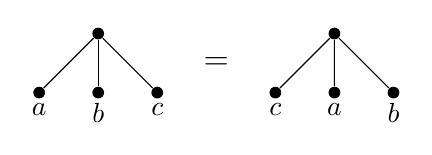
\begin{tikzpicture}[scale=0.75, every node/.style={inner sep=1.5pt}]
    \node (r1) at (0,0) [circle,fill,minimum size=4pt] {};
    \node (a1) at (-1,-1) [circle,fill,minimum size=4pt,label=below:$a$] {};
    \node (b1) at (0,-1) [circle,fill,minimum size=4pt,label=below:$b$] {};
    \node (c1) at (1,-1) [circle,fill,minimum size=4pt,label=below:$c$] {};
    \draw (r1) -- (a1);
    \draw (r1) -- (b1);
    \draw (r1) -- (c1);

    \node at (2, -0.5) {\large $=$};

    \node (r2) at (4,0) [circle,fill,minimum size=4pt] {};
    \node (c2) at (3,-1) [circle,fill,minimum size=4pt,label=below:$c$] {};
    \node (a2) at (4,-1) [circle,fill,minimum size=4pt,label=below:$a$] {};
    \node (b2) at (5,-1) [circle,fill,minimum size=4pt,label=below:$b$] {};
    \draw (r2) -- (c2);
    \draw (r2) -- (a2);
    \draw (r2) -- (b2);
  \end{tikzpicture}
  \end{center}

  \note{%
    Timing: 1:30.

    This is the motivating example.

    A symmetric tree is a tree where the order of the children does not matter.

    We consider the branching factor to be infinite, say $\mathbb{N}$, so each
    node has one child position for each natural number.

    The equation says that if we permute the children, we get the same
    tree.

    The picture only shows finitely many children, but it gives the right
    intuition: order is not supposed to matter.
  }
\end{frame}

% ---------------------------------------------------------------------------
% Slide 9: The obvious construction
% ---------------------------------------------------------------------------
\begin{frame}{The obvious construction}
  Start with raw ordered trees \(W\).

  \[
    \ell_W : W
    \qquad
    n_W : (\mathbb N \to W) \to W
  \]

  \medskip

  Then quotient by permutation:

  \[
    Q := W/{\sim}
  \]

  \medskip

  Question:

  \begin{center}
    \large
    Is \(Q\) really the quotient inductive type of symmetric trees?
  \end{center}

  \note{%
    Timing: 1:00.

    The obvious construction is to start with the ordinary type of ordered
    trees.

    Then we quotient by the relation that permutes children.

    At the level of elements, this looks right.

    The question is whether this quotient carries the right constructor
    structure.

    In other words, does it really behave as the quotient inductive type
    of symmetric trees?
  }
\end{frame}

% ---------------------------------------------------------------------------
% Slide 10: The lifting problem
% ---------------------------------------------------------------------------
\begin{frame}[fragile]{Why the obvious construction fails}
  The leaf constructor lifts immediately:

  \[
    \widetilde{\ell} := [\ell_W].
  \]

  \medskip

  But for nodes we need:

  \[
    \widetilde n : Q^{\mathbb N} \to Q
  \]

  \[
  \begin{tikzcd}
    Q^{\mathbb N}
      \arrow[d, dashed, "choose representatives"']
      \arrow[rr, dashed, "\widetilde n"] &&
    Q \\
    W^{\mathbb N} \arrow[r, "n_W"'] &
    W \arrow[ur, "{[-]_\sim}"']
  \end{tikzcd}
  \]

  \begin{center}
    \large
    A quotient gives classes, but a constructor wants representatives.
  \end{center}

  \note{%
    Timing: 2:00.

    This is the central obstruction.

    The leaf is easy: we just take the equivalence class of the raw leaf.

    But the node constructor is different.

    Its input is a family of quotient elements, not a family of raw trees.

    To apply the raw constructor, we would need to choose a representative
    tree for every input.

    For finitely many inputs this is not a serious problem, but for
    countably many inputs this is exactly the shape of a choice problem.

    So this is the slogan: a quotient gives classes, but a constructor
    wants representatives.
  }
\end{frame}

% ---------------------------------------------------------------------------
% Slide 11: Existing approach
% ---------------------------------------------------------------------------
\begin{frame}{The existing approach}
  \begin{columns}[T]
    \begin{column}{0.55\textwidth}
      Fiore, Pitts, and Steenkamp (FPS) construct infinitary QITs stagewise.

      \begin{enumerate}
        \item build depth-bounded approximations \(D_\alpha\)
        \item quotient each stage
        \item take \(Q := \mathrm{colim}\,D\)
      \end{enumerate}
      \medskip
    \end{column}
    \begin{column}{0.45\textwidth}
      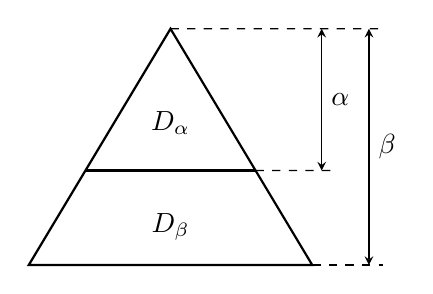
\begin{tikzpicture}[scale=0.6, thick, text=black, draw=black]

        % Define the main vertices
        \coordinate (Top) at (0, 5);
        \coordinate (BottomLeft) at (-3, 0);
        \coordinate (BottomRight) at (3, 0);

        % Draw the main outer triangle (D_\beta boundary)
        \draw (BottomLeft) -- (BottomRight) -- (Top) -- cycle;

        % Define and draw the horizontal subdivision line
        % This partitions the triangle at y=2
        \coordinate (MidLeft) at (-1.8, 2);
        \coordinate (MidRight) at (1.8, 2);
        \draw (MidLeft) -- (MidRight);

        % Place the labels inside their respective regions
        \node at (0, 3) {$D_\alpha$};
        \node at (0, 0.8) {$D_\beta$};

        % Draw thin, dashed guide lines for the vertical dimensions
        \draw[dashed, thin] (Top) -- (4.5, 5);
        \draw[dashed, thin] (MidRight) -- (3.5, 2);
        \draw[dashed, thin] (BottomRight) -- (4.5, 0);

        % Add the vertical dimension arrows and corresponding labels
        \draw[<->, >=stealth, thin] (3.2, 2) -- node[right] {$\alpha$} (3.2, 5);
        \draw[<->, >=stealth, thin] (4.2, 0) -- node[right] {$\beta$} (4.2, 5);

      \end{tikzpicture}
    \end{column}
  \end{columns}

  The hard step is showing that constructors still work at the limit.

  \medskip

  \begin{center}
    \large
    This is where a weak form of choice is used.
  \end{center}

  \note{%
    Timing: 1:30.

    There is a known general approach, due to Fiore, Pitts, and Steenkamp.

    The idea is to avoid choosing all representatives at once by building
    the type in stages.

    At each stage, only bounded information is allowed.

    Then the stages are assembled into a limiting object.

    The hard part is showing that the constructors still work after taking
    that limit.

    In the general proof, this is where a weak form of choice is used.
  }
\end{frame}

% ---------------------------------------------------------------------------
% Slide 12: My observation
% ---------------------------------------------------------------------------
\begin{frame}{The key property}
  In symmetric trees, permutation does not change depth.

  \medskip

  \begin{center}
  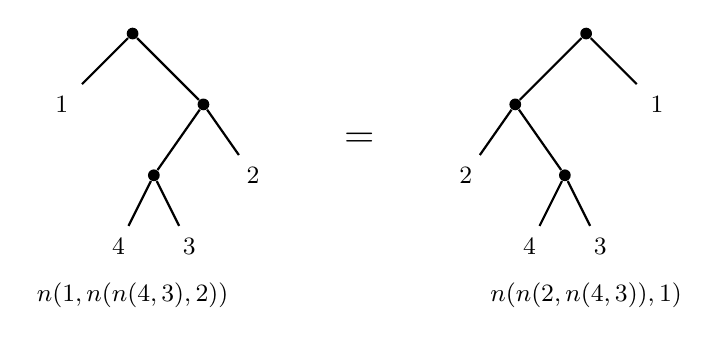
\begin{tikzpicture}[
    scale=0.9,
    every node/.style={font=\small},
    internal/.style={circle, fill, inner sep=1.5pt},
    leaf/.style={minimum size=5mm, inner sep=0pt},
    edge/.style={thick}
  ]

  % ---------------------------------------------------------------------------
  % Left tree: n(1,n(n(4,3),2))
  % ---------------------------------------------------------------------------

  \node[internal] (Lroot) at (0,0) {};
  \node[leaf]     (L1)    at (-1,-1) {$1$};
  \node[internal] (Lr)    at (1,-1) {};

  \node[internal] (Lrl)   at (0.3,-2) {};
  \node[leaf]     (L2)    at (1.7,-2) {$2$};

  \node[leaf]     (L4)    at (-0.2,-3) {$4$};
  \node[leaf]     (L3)    at (0.8,-3) {$3$};

  \draw[edge] (Lroot) -- (L1);
  \draw[edge] (Lroot) -- (Lr);
  \draw[edge] (Lr) -- (Lrl);
  \draw[edge] (Lr) -- (L2);
  \draw[edge] (Lrl) -- (L4);
  \draw[edge] (Lrl) -- (L3);

  \node at (0,-3.7) {$n(1,n(n(4,3),2))$};

  % Equality sign
  \node at (3.2,-1.5) {\Large $=$};

  % ---------------------------------------------------------------------------
  % Right tree: n(n(2,n(4,3)),1)
  % ---------------------------------------------------------------------------

  \node[internal] (Rroot) at (6.4,0) {};
  \node[internal] (Rl)    at (5.4,-1) {};
  \node[leaf]     (R1)    at (7.4,-1) {$1$};

  \node[leaf]     (R2)    at (4.7,-2) {$2$};
  \node[internal] (Rlr)   at (6.1,-2) {};

  \node[leaf]     (R4)    at (5.6,-3) {$4$};
  \node[leaf]     (R3)    at (6.6,-3) {$3$};

  \draw[edge] (Rroot) -- (Rl);
  \draw[edge] (Rroot) -- (R1);
  \draw[edge] (Rl) -- (R2);
  \draw[edge] (Rl) -- (Rlr);
  \draw[edge] (Rlr) -- (R4);
  \draw[edge] (Rlr) -- (R3);

  \node at (6.4,-3.7) {$n(n(2,n(4,3)),1)$};

  \end{tikzpicture}
  \end{center}

  \medskip

  Permutation changes order, but not how far down the tree each subtree is.

  \medskip

  \begin{center}
    \large
    Equality preserves stage.
  \end{center}

  \note{%
    Timing: 1:30.

    The key observation is that the equations for symmetric trees preserve depth.

    A permutation changes the order of the children, but it does not move a
    subtree higher or lower in the tree.

    That means that if two trees are identified by the symmetric tree equations,
    they should appear at the same stage of the construction.

    This is the special feature that makes symmetric trees better behaved than the
    general case.
  }
\end{frame}

% ---------------------------------------------------------------------------
% Slide 13: Ordinal basis
% ---------------------------------------------------------------------------
\begin{frame}{What extra structure is needed?}
  To make the stage assignment well behaved, I assume an
  \emph{extensional ordinal basis}.

  \medskip

  Informally, this is a supply of stages satisfying:

  \begin{itemize}
    \item every constructor has a stage
    \item stages are ordered by ``being below''
    \item stages that have the same predecessors are identified
  \end{itemize}

  \medskip

  This is weaker than assuming the whole quotient inductive type exists.

  \note{%
    Timing: 1:30.

    To make this argument precise, I assume an extensional ordinal basis.

    This is the technical extra structure in my result.

    Informally, it gives a supply of stages closed under the constructors
    we need.

    It also has an extensionality principle: stages are determined by the
    stages below them.

    This is not the same as assuming the quotient inductive type already
    exists.

    It is a more specific ordinal principle that is enough for the symmetric tree
    case.
  }
\end{frame}

% ---------------------------------------------------------------------------
% Slide 14: Result
% ---------------------------------------------------------------------------
\begin{frame}{My result}
  For symmetric trees, depth preservation gives a stable stage assignment.

  \medskip

  Therefore the stagewise construction can be carried out relative to an
  extensional ordinal basis.

  \medskip

  \begin{center}
    \large
    The full weak-choice argument is not needed in the same way as in the
    general construction.
  \end{center}

  \medskip

  Partially formalised in Agda.

  \note{%
    Timing: 1:30.

    This is the main result I want to communicate.

    For symmetric trees, depth preservation gives enough control to assign stages
    coherently.

    That lets us recover the stagewise construction relative to an
    extensional ordinal basis.

    So the general weak-choice argument is not needed in the same way for
    this example.

    I have partially formalised this argument in Agda.
  }
\end{frame}

% ---------------------------------------------------------------------------
% Slide 15: Why this does not solve everything
% ---------------------------------------------------------------------------
\begin{frame}{Why this does not solve everything}
  It is tempting to look for a broad syntactic criterion.

  \medskip

  For example:
  \begin{itemize}
    \item equations preserve depth
    \item equations only inspect bounded depth
  \end{itemize}

  \medskip

  But boundedness alone is not enough.

  \medskip

  Some examples still require large ordinal strength or choice-like
  principles.

  \note{%
    Timing: 1:30.

    The natural next question is whether this generalises.

    Depth preservation is syntactic: we can read it directly from the
    equations.

    So one might hope for a broad syntactic criterion, such as bounded
    depth or locality.

    But boundedness alone cannot be the whole story.

    Even if equations have a bounded form, the ordinal structure required
    to interpret all derived witnesses may itself be hard to construct.

    Known examples show that the general problem still has real ordinal
    strength.
  }
\end{frame}

% ---------------------------------------------------------------------------
% Slide 16: Future work
% ---------------------------------------------------------------------------
\begin{frame}{Where next?}
  Working conjecture:

  \medskip

  \begin{center}
    \large
    symmetric trees are not derivable from quotients and \(W\)-types alone,
    without an additional ordinal principle.
  \end{center}

  \medskip

  Next steps:
  \begin{itemize}
    \item Construct a model of algebraic set theory that has quotients, but not symmetric treeo
    \item Construct a larger class of QITs from a minimal choice principle
  \end{itemize}

  \note{%
    Timing: 1:30.

    My current working conjecture is that the extra ordinal basis is not
    merely an artefact of the proof.

    In other words, symmetric trees are probably not derivable from quotients and
    W-types alone, without an additional ordinal principle.

    The next step is to refute this by finding a model of type theory
    which as quotients and W-types but not symmetric trees.

    I also want to complete the Agda formalisation and test the boundary
    on more examples.

    The bigger aim is to understand which structural features of equations
    force choice-like strength.
  }
\end{frame}

% ---------------------------------------------------------------------------
% Slide 17: Conclusion
% ---------------------------------------------------------------------------
\begin{frame}{Takeaway}
  \begin{itemize}
    \item Quotients forget representatives.
    \item Constructors may need representatives back.
    \item In infinitary cases, this becomes choice-shaped.
    \item symmetric trees are a positive test case because equality preserves depth.
    \item The general boundary is still open.
  \end{itemize}

  \medskip

  \begin{center}
    \large
    The syntax of the equations matters.
  \end{center}

  \note{%
    Timing: 1:00.

    The takeaway is this.

    Quotients forget representatives.

    But constructors may need representatives back.

    In infinitary cases, recovering those representatives becomes
    choice-shaped.

    symmetric trees are a useful positive test case because their equations
    preserve depth.

    But the general boundary remains open.

    The syntax of the equations matters, and understanding exactly how is
    the next stage of the project.
  }
\end{frame}

\begin{frame}[allowframebreaks]{References}
  \tiny
  \begin{thebibliography}{3}

  \bibitem{abbott2005-containers}
  Michael Abbott, Thorsten Altenkirch, and Neil Ghani.
  \newblock Containers: Constructing strictly positive types.
  \newblock {\em Theoretical Computer Science}, 342(1):3--27, 2005.

  \bibitem{altenkirch2016-qit}
  Thorsten Altenkirch and Ambrus Kaposi.
  \newblock Type theory in type theory using quotient inductive types.
  \newblock In {\em Proceedings of the 43rd ACM SIGPLAN-SIGACT Symposium on
    Principles of Programming Languages (POPL 2016)}, pages 18--29, 2016.

  \bibitem{altenkirch2018-qiit}
  Thorsten Altenkirch, Paolo Capriotti, Gabe Dijkstra, Nicolai Kraus, and
  Fredrik Nordvall Forsberg.
  \newblock Quotient inductive-inductive types.
  \newblock In {\em Foundations of Software Science and Computation Structures
    (FoSSaCS 2018)}, pages 293--310, 2018.

  \bibitem{altenkirch2017-partiality-monad}
  Thorsten Altenkirch, Nils Anders Danielsson, and Nicolai Kraus.
  \newblock Partiality, revisited: The partiality monad as a quotient inductive-inductive type.
  \newblock In {\em Foundations of Software Science and Computation Structures (FoSSaCS 2017)}, pages 17--33, 2017.

  \bibitem{blass1983-words}
  Andreas Blass.
  \newblock Words, free algebras, and coequalizers.
  \newblock {\em Fundamenta Mathematicae}, 117(3):255--256, 1983.

  \bibitem{fiore2022-quotients-inductive-types}
  Marcelo P.~Fiore, Andrew M.~Pitts, and S.~C.~Steenkamp.
  \newblock Quotients, inductive types, and quotient inductive types.
  \newblock {\em Logical Methods in Computer Science}, 18(2), 2022.

  \bibitem{kaposi2019-constructing}
  Ambrus Kaposi, Andr\'as Kov\'acs, and Thorsten Altenkirch.
  \newblock Constructing quotient inductive-inductive types.
  \newblock {\em Proceedings of the ACM on Programming Languages},
    3(POPL):2:1--2:24, 2019.

  \bibitem{kaposi2021-setoid}
  Ambrus Kaposi and Zongpu Xie.
  \newblock Quotient inductive-inductive types in the setoid model.
  \newblock In {\em 27th International Conference on Types for Proofs and
    Programs (TYPES 2021)}, presentation abstract/slides, 2021.

  \bibitem{kovacs2020-large}
  Andr\'as Kov\'acs and Ambrus Kaposi.
  \newblock Large and infinitary quotient inductive-inductive types.
  \newblock In {\em Proceedings of the 35th Annual ACM/IEEE Symposium on Logic in
    Computer Science (LICS 2020)}, pages 648--661, 2020.

  \bibitem{kraus2023-ordinal}
  Nicolai Kraus, Fredrik Nordvall Forsberg, and Chuangjie Xu.
  \newblock Type-theoretic approaches to ordinals.
  \newblock {\em Theoretical Computer Science}, 957:113843, 2023.

  \bibitem{lumsdaine2020-hit}
  Peter LeFanu Lumsdaine and Michael Shulman.
  \newblock Semantics of higher inductive types.
  \newblock {\em Mathematical Proceedings of the Cambridge Philosophical
    Society}, 169(1):159--208, 2020.

  \bibitem{taylor1996-intuitionistic}
  Paul Taylor.
  \newblock Intuitionistic sets and ordinals.
  \newblock {\em The Journal of Symbolic Logic}, 61(3):705--744, 1996.

  \bibitem{hott2013-book}
  The Univalent Foundations Program.
  \newblock Homotopy Type Theory: Univalent Foundations of Mathematics.
  \newblock Institute for Advanced Study, 2013.

  \bibitem{vandenberg2012-wisc-axiom}
  Benno van den Berg and Ieke Moerdijk.
  \newblock The axiom of multiple choice and models for constructive set theory.
  \newblock {\em arXiv preprint arXiv:1204.4045}, 2012.

  \end{thebibliography}
\end{frame}

\begin{frame}
  \centering
  \vfill
  {\LARGE Thank you for listening}

  \vspace{1em}

  Questions?
  \vspace{1em}
  Links:
  \begin{itemize}
    \item Agda Source: \url{https://github.com/cdo256/agda-qit}
    \item My website on type theory: \url{https://octocurious.com}
  \end{itemize}
  \vfill
  \note{%
  }
\end{frame}

\end{document}
